\chapter{Baggrund For Projektet}
\label{Background}

\section{Booking på ITU}
\label{Background_Book}
IT-Universitet er et stort universitet med mange ressourcer, som de studerende og ansatte kan benytte sig af, der er derfor behov for et system der kan understøtte booking af lokaler, udstyr og forplejning.

I øjeblikket er booking af ressourcer på ITU et uoverskueligt og problemfyldt område. Planlægningen af de forskellige ressourcer sker i dag primært manuelt i mange forskellige systemer hvor Facility Management (FM) fungerer som centralt bindepunkt for alt vedrørende lokale administration. Dette er ikke holdbart, da systemet ikke giver nok gennemskuelighed i forhold til at bruge ressourcerne i systemet bedre. Da meget af arbejdet sker manuelt skal personalet opretter alle bookinger, meget af deres tid bruges derfor på arbejdesopgaver som brugeren skulle udføre selv. 

Det udfordrende ved at lave et automatiseret booking system til IT-Universitet er, at det skal understøtte bookinger af de forskellige ressourcer. Det skal derfor understøtte mange arbejdsområder, og der skal tages hensyn til mange forskellige aktører, eksemepelvis studerende, ansatte og kantinemedarbejder.

 For at have overblik over, hvad der skulle understøttes og hvad der var vigtigst fulgte vi en kravspecifikation som blev udarbejdet i kurset "Anskaffelse og kravspecifikation" på ITU i efteråret 2012, skrevet af Stig Larsen (stla@itu.dk), Miki Ipsen (mikc@itu.dk), Garwun Jeffrey Lai (gjel@itu.dk) og Merete Larsen (mnol@itu.dk). Kravspecifikationen er lavet med fokus specifikt på ITU og hvad et bookingsystem til ITU kræver.

\section{Kravspecifikationen}
\label{Background_Kravspec}
Som nævnt er kravspecifikationen specifikt udviklet med henblik på hvad der kræves af et bookingsystem på IT-Universitet. Den giver derfor et overblik og hvordan bookingen af ressourcer fungerer i øjeblikket. Figur \ref{Baggrund_Kravspec_NuvaerendeFlow} viser den nuværende situation.

\begin{figure}[h!]
  \centering
    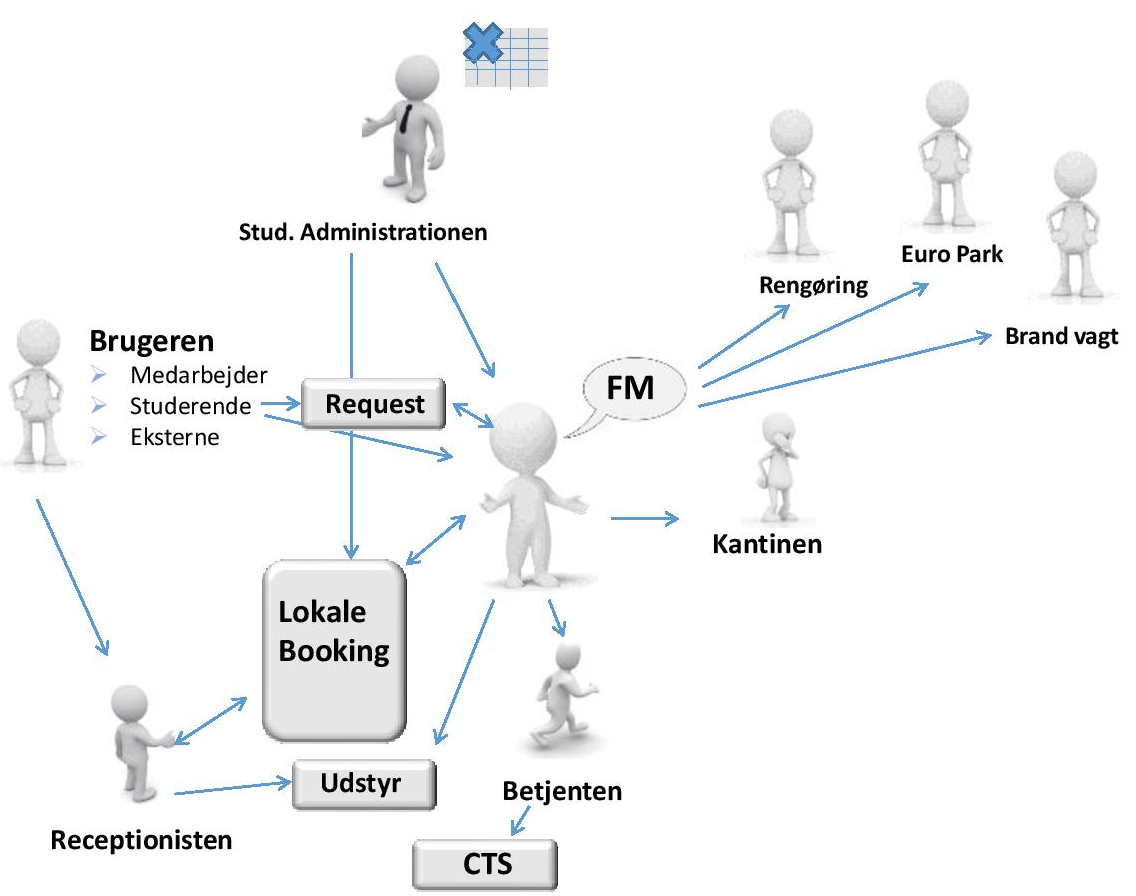
\includegraphics[width=0.7\textwidth]{Appendix/GUI-Prototype/NuvaerendeFlow}
  \caption{Nuværende system flow for booking systemet på ITU}
\label{Baggrund_Kravspec_NuvaerendeFlow}
\end{figure}

For at forbedre den nuværende løsning foreslår kravspecifikationen, at der laves et systemet som alle aktører arbejder op imod.
Figur \ref{Baggrund_Kravspec_DesiredFlow} 

\begin{figure}[h!]
  \centering
    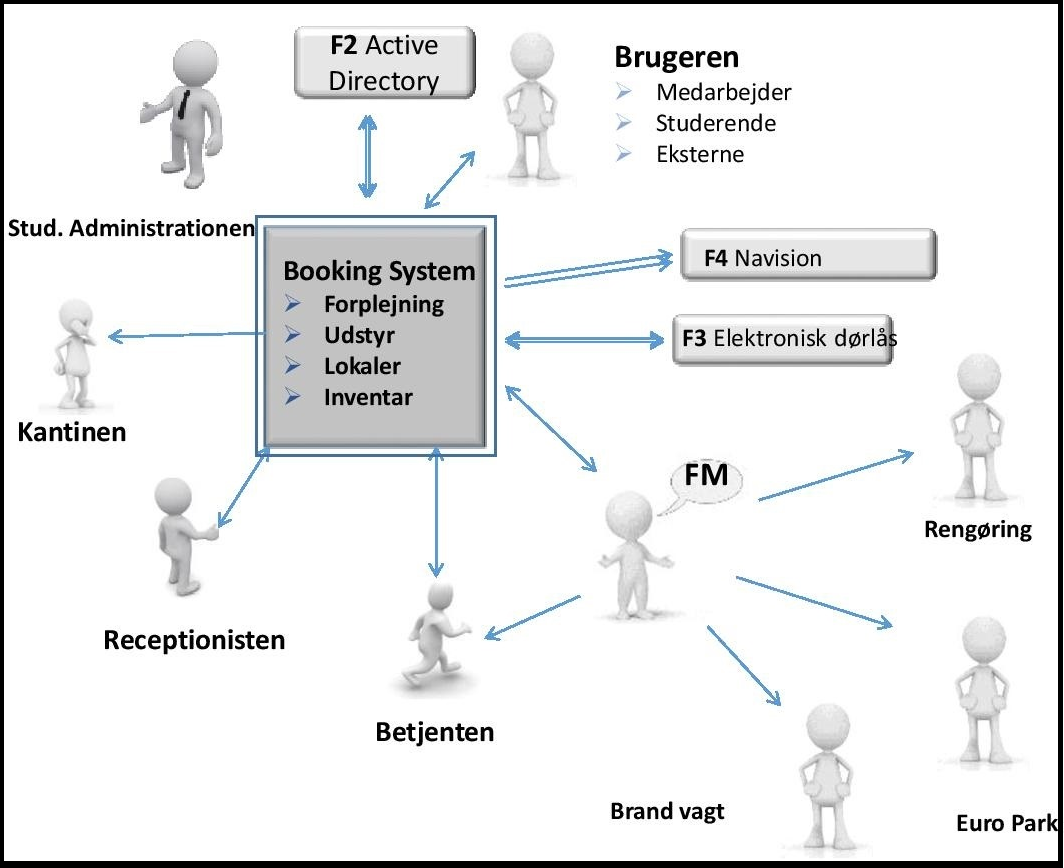
\includegraphics[width=0.7\textwidth]{Appendix/GUI-Prototype/DesiredFlow}
  \caption{Det ønskede system flow for booking systemet på ITU}
\label{Baggrund_Kravspec_DesiredFlow}
\end{figure}

Til udviklingen af det nye system definerer kravspecifikationen 13 arbejdsopgaver som udgør den funktionalitet der kræves af det nye system. Hvis alle 13 arbejdsopgaver bliver understøtte vil det nye system løse problemerne med gennemskueligheden i forhold til ressourcerne, derudover vil brugeren kunne lave mange af arbejdsopgaverne, og det vil derfor også løse problemet med at de ansatte brugere for meget tid på at oprette bookinger.

\section{Problemformulering}
\label{Background_Problem}
Vi vil til projektet udvikle et booking system til IT-Universitet  som er basseret på kravspecifikationens 13 arbejdsopgaver. Vi har i den sammenhæng fire hovedpunkter.
\begin{my_itemize}
\item {}
\item {}
\item {}
\item {}
\item {}
\end{my_itemize}
Vi vil udvikle et booking system til IT-Universitet  som er basseret på kravspecifikationens 13 arbejdsopgaver. Vi vil udvikle en webservice og en browser klient som benytter sig af webservicen.


for projektet ligger vores problemformulering.
Vi vil udvikle et booking system til IT-universitetet baseret på kravspecifikationen "ITU booking system". Vi vil til det formål udvikle en webservice der undersøtter cross-platform, vi vil samtidig udvikle en klient som benytter sig af webservicen. Vi vil derudover vurdere om hvorvidt vores løsning opfylder kravspecifikationen og i hvilken grad, desuden vi vil undersøge om der allerede findes systemeret på markedet som kan det samme eller eller mere, som vores produkt.